% Homework template for Algorithm Analysis and Design
% UPDATE: September 20, 2019 by Xu Rongchen
\documentclass[a4paper]{article}
\usepackage{ctex}
\ctexset{
proofname = \heiti{证明} %% set proof name
}
\usepackage{amsmath, amssymb, amsthm}
% amsmath: equation*, amssymb: mathbb, amsthm: proof
\usepackage{moreenum}
\usepackage{mathtools}
\usepackage{url}
\usepackage{bm}
\usepackage{enumitem}
\usepackage{graphicx}
\usepackage{subcaption}
\usepackage{booktabs} % toprule
\usepackage[mathcal]{eucal}

\usepackage{iidef} % set homework count
\usepackage{longtable}

% \usepackage[noend]{algpseudocode}
\usepackage{clrscode3e}

\thecoursename{算法分析与设计实验报告}
\theterm{2019年秋季学期}
\hwname{Seam Carving实现}
\slname{\heiti{解}}
\begin{document}
\courseheader
\theusername{徐荣琛}
\thestuno{2019214518}
\theinstitute{软件学院}

\info

\begin{enumerate}
  \setlength{\itemsep}{3\parskip}
  \textbf{1.实验要求}\\
  实验要求有算法设计描述以及伪码。同时具体实现一个将图片进行Seam Carving压缩的程序,
  程序的基本功能是可以讲$m\times n$的图像压缩为$m/2 \times n/2$,并有方便的输入
  输出功能,其它功能不限,提交实验报告。\\
  \bigskip

  \textbf{2.实验环境}\\
  此次实验代码采用C\#语言实现,具体的实验环境及编译配置如下表所示:\\ \medskip
  \begin{tabular}{c|c}
    \hline\hline
    处理器 & Intel(R) Core(TM) i7-8850H CPU @ 2.60GHz \\ \hline
    内存 & 16GB\\ \hline
    操作系统& Mac OS X 10.14.6\\ \hline
    编译环境& .Net Core 3.0.100\\
    \hline\hline
  \end{tabular}\\
  \bigskip

  \textbf{3.实验内容}\\
  \textbf{3.1 算法的设计}\\
  \medskip
  Seam Carving 算法分为4个主要的步骤:\\
  (1)像素点能量值计算,具体计算策略在下一节详细介绍;\\
  (2)根据(1)中像素点能量值,使用动态规划的策略计算出水平方向(或垂直方向)上的一条像素路径,使得这条
  路径的能量值之和在所有水平方向(或垂直方向)的路径中最小;\\
  (3)删除这条路径上的所有像素点,将两侧的点相连,并在连接缝隙处做一定的平滑化处理;\\
  (4)重复(1)至(3)的步骤,直至图片的尺寸与目标尺寸一致。\\
  算法的伪代码如下:\\
  % \resizebox{\linewidth}{!}{ 
    \newcommand{\Doo}{\>\textbf{}\hspace*{-0.7em}\'\addtocounter{indent}{1}}
    \begin{minipage}{320pt}
    \begin{codebox}
        \Procname{$\proc{Seam-Carving}$($pic$, $height$, $width$)}
        \li \While $pic.height > height$
            \Doo 
        \li     $E = \proc{Calculate-Energy}(pic)$
        \li     $BestRouteH = \proc{Find-Best-Route-H}(E)$
        \li     $pic.Remove(BestRouteH)$
            \End
        \li \While $pic.width > width$
            \Doo 
        \li     $E = \proc{Calculate-Energy}(pic)$
        \li     $BestRouteW = \proc{Find-Best-Route-W}(E)$
        \li     $pic.Remove(BestRouteW)$
            \End
        \li \Return $pic$
    \end{codebox}
\end{minipage}\\
% }\\ 
  \medskip
  \textbf{3.2 能量值策略}\\
  \medskip
  Seam Carving算法之中,像素点能量值的形象化含义即改像素点与周围像素点的差异,而算法的思路即是去除图片上
  差异值最小的一条路径。在此,采用梯度的概念来量化这个差异。\\
  首先人为地认为像素的能量值即这个像素点在RGB三个通道上的能量值简单相加,对于每个通道上的能量值,采用以下
  矩阵卷积的形式来近似垂直向的梯度$E_1 = |Conv(M,D)|$,其中$Conv$是卷积操作,$M$是图片通道矩阵,卷积核$D$
  如下所示:
  $$ D =
  \left[
  \begin{matrix}
    1 & 2 & 1 \\
    0 & 0 & 0 \\
    -1 & -2 & -1
  \end{matrix}
  \right]
  $$
  相应地,水平向的梯度$E_2 = |Conv(M,D^T)|$,这样像素点的能量值矩阵$E = E_1 + E_2$。\\
  由于卷积会导致矩阵缩小,为了保证所有点均能获得一个能量值,在卷积开始前对原矩阵进行扩维,即在原矩阵对四周
  填充一圈0值(亦可填充临近的边缘值,但结果表明差异并不明显)。\\
  \medskip
  \textbf{3.3 动态规划求最佳路径}\\
  \medskip
  以水平方向为例。算法自左向右进行动态规划($x$增大),设定二维数组$DP$与当前图片大小一致,
  初始$DP[0][i]=E[0][i]$,之后向右遍历,则:
  $$DP[x][i]= \min(DP[x-1][i-1],DP[x-1][i],DP[x-1][i+1])+ E[x][i]$$
  特别地,如果$i$是边界值,只需考虑左侧两个像素点中但较小值即可。\\
  最后,遍历最右侧的一列值,其中的最小值即最优能量值之和。这样每次的最佳路径求解即可在
  $O(height*widht)$的时间复杂度下求解。\\
  注意,由于需要得到具体的路径,在每次计算中还需要额外记录当前最小值的来源$(+1,0,-1)$,这样从最后的
  最优解位置可以反向获得最优解的路径。\\
  \medskip
  \textbf{3.4 复杂度分析和实现改进}\\
  由于需要将图片的长宽均缩小一半,所以整个算法的时间复杂度为$O(height*widht*\max(height,widht))$,
  考虑到过程中还包含来一系列的较复杂的矩阵卷积运算,所以时间复杂度的常数也会较大,对于较大的图片(1080P以上),
  实验速度较慢,为了缩短图片生成时间,考虑到矩阵运算的可并行性,代码实现时在相关矩阵运算的时候使用了多线程计算,
  这样很大程度上加速了图片生成的效率。\\
  \textbf{3.5 实验效果和分析}\\
  实验效果(左侧为原图,右侧为裁剪后的图片):\\
  风景图片效果:
  

  \begin{center}
    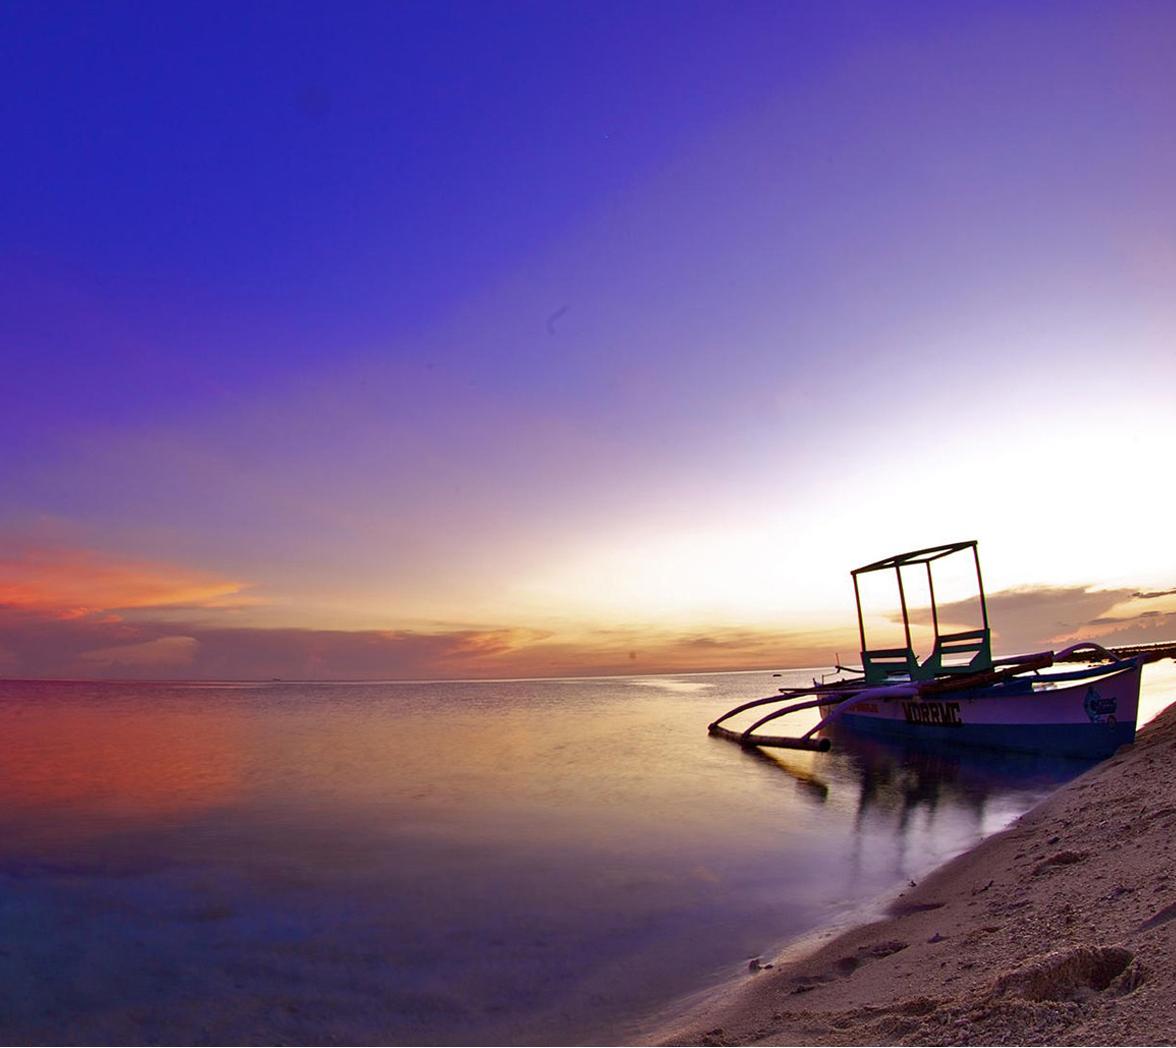
\includegraphics[scale=0.125]{Pictures/example52}
    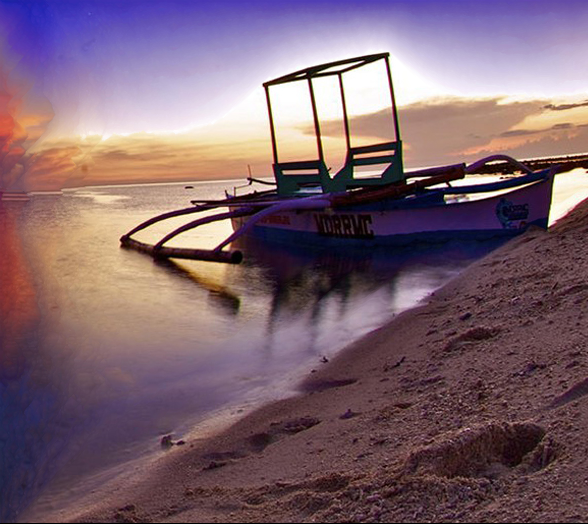
\includegraphics[scale=0.25]{Pictures/er52nm.jpg}
  \end{center}
  星空图片效果:


  \begin{center}
    
\includegraphics[scale=0.075]{Pictures/example2.jpg}
    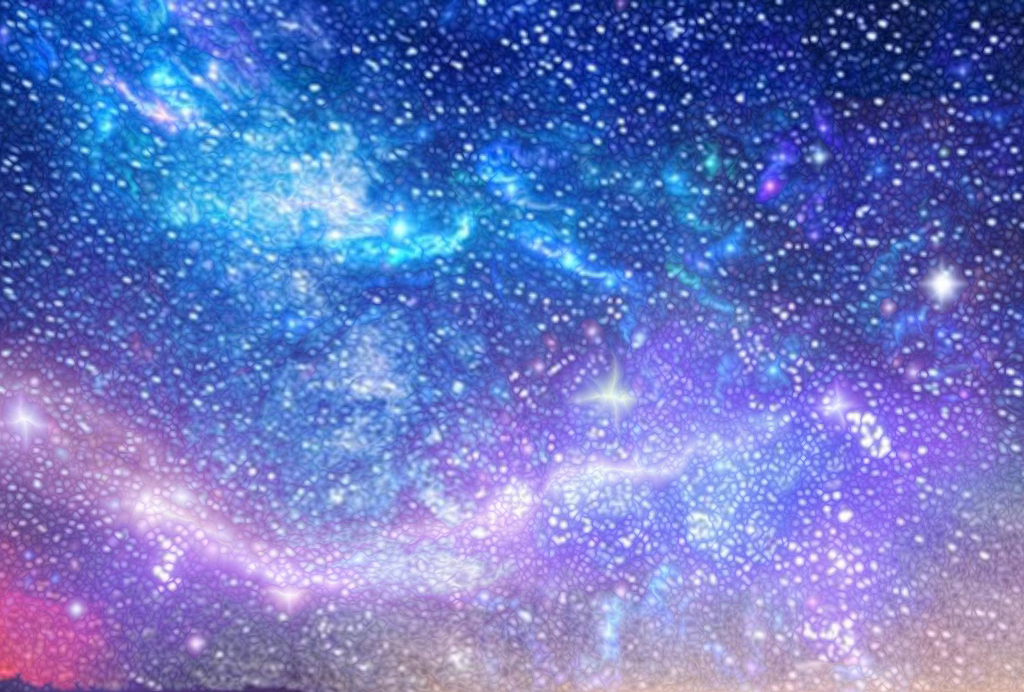
\includegraphics[scale=0.15]{Pictures/er2n.jpg}
  \end{center}
  
  对于类似上述图片的一些图片,Seam Carving算法表现出了优异的效果,在保持主要元素尺寸的不发生变化的条件下
  缩小了次要内容的空间。一般地发现,当图片存在较大空当时,算法表现显著优于不存在空当的图片。\\
  但是实际其它实验效果表明,Seam Carving算法也有表现不佳的一些情况,经过总结主要包括以下一些原因:\\
  (1)经过裁剪的元素内部尺寸比例可能发生变化;\\
  (2)裁剪导致边缘变形的发生(例如原有的直线可能变弯)。
\end{enumerate}
\end{document}